\section{Quadratic Unconstrained Binary Optimization (QUBO) and Ising Model}
The following content is from the tutorial held by D-Wave \cite{DWAVE_Tutorial}. In the context of D-Wave's quantum annealing, QUBO and the Ising model are the two primary mathematical frameworks used to formulate optimization problems. Both are unified under the broader category of \textbf{Binary Quadratic Models (BQM)}.
QUBO model can be used to a wide range of optimization problems, including combinatorial optimization, machine learning, and constraint satisfaction problems. The QUBO formulation is particularly useful in quantum computing and optimization, as it can be directly mapped to the hardware of quantum annealers like those developed by D-Wave.
QUBO is a mathematical representation of an optimization problem where the objective function is a quadratic polynomial of binary variables. The goal is to find the assignment of these binary variables that minimizes (or maximizes) the objective function. 
Unconstrained means that there are no explicit constraints on the variables, allowing for a more flexible formulation of problems. The QUBO formulation is particularly useful in quantum computing and optimization, as it can be directly mapped to the hardware of quantum annealers like those developed by D-Wave.
\subsection{QUBO Formulation}
Because $x^2 = x$ for binary variables, the QUBO formulation can be expressed as:
\begin{equation}
\min_{x \in \{0,1\}^n} x^T Q x
\label{eqn:qubo}
\end{equation}
where $x$ is a vector of binary variables, and $Q$ is an upper triangular matrix that defines the coefficients of the quadratic terms. The elements of $Q$ represent the interactions between the binary variables, and the diagonal elements represent the linear terms.
Here are some specific examples of QUBO formulations for numbers of varaibles:
\begin{itemize}
\item One-variable QUBO: $Q = [1]$, the objective function is $f(x) = x$.
\item Two-variable QUBO: $Q = \begin{bmatrix} 1 & 2 \\ 0 & 3 \end{bmatrix}$, the objective function is $f(x_1, x_2) = x_1 + 2x_1x_2 + 3x_2$.
\item Three-variable QUBO: $Q = \begin{bmatrix} 1 & 2 & 3 \\ 0 & 4 & 5 \\ 0 & 0 & 6 \end{bmatrix}$, the objective function is $f(x_1, x_2, x_3) = x_1 + 2x_1x_2 + 3x_1x_3 + 4x_2 + 5x_2x_3 + 6x_3$.
\end{itemize}
It is easy to see that the number contained in the QUBO matrix $Q$ corresponds to the coefficients of the objective function. In contrast, the following examples are NOT QUBOs:
\begin{itemize}
    \item $f(x_1) = 3x_1 + 4 + x_1^3$
    \item $f(x_1, x_2) = 11 + 2.7x_1 - 3x_2 + 9.3x_1/x_2$
    \item $f(x_1, x_2, x_3) = x_1x_2x_3$
\end{itemize}
Except for the $Q$ matrix, the QUBO can also be represented in a graphical form, where each variable is represented as a node, and the edges denote the interactions between the variables. The weights of the edges correspond to the coefficients in the QUBO matrix. This graphical representation can be useful for visualizing the structure of the optimization problem and understanding the relationships between the variables. Figure \ref{fig:qubo_graph} is an example of a QUBO graph for the three-variable case $f(x_1, x_2, x_3)=x_1 + 2x_1x_2 + 3x_1x_3 + 4x_2 + 5x_2x_3 + 6x_3$. In this graph, constant terms and variable names are omitted, and the weights of the edges are labeled. The nodes represent the binary variables $x_1$, $x_2$, and $x_3$, while the edges represent the interactions between these variables, with their weights corresponding to the coefficients in the QUBO matrix.
\begin{figure}
    \centering
    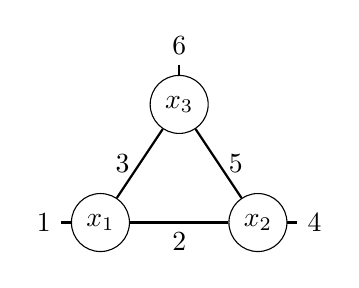
\begin{tikzpicture}
        \node[circle, draw] (x1) at (0, 0) {$x_1$};
        \node[circle, draw] (x2) at (2, 0) {$x_2$};
        \node[circle, draw] (x3) at (1, 1.5) {$x_3$};

        \draw[thick] (x1) -- (x2) node[midway, below] {2};
        \draw[thick] (x1) -- (x3) node[midway, left] {3};
        \draw[thick] (x2) -- (x3) node[midway, right] {5};

        \draw[thick] (x1) -- ++(-0.5, 0) node[left] {1};
        \draw[thick] (x2) -- ++(0.5, 0) node[right] {4};
        \draw[thick] (x3) -- ++(0, 0.5) node[above] {6};
    \end{tikzpicture}
    \caption{Example of a QUBO graph}\label{fig:qubo_graph}
\end{figure}

\subsection{Ising Model}
The Ising model is a mathematical model used to describe the behavior of ferromagnetic materials. It is closely related to the QUBO formulation and can be used to represent optimization problems in a different but equivalent way. In the Ising model, the variables are spins that can take values of either +1 or $-1$, and the interactions between spins are represented by coupling constants. The goal is to find the configuration of spins that minimizes the energy of the system. 
The mathematical representation of the Ising model can be expressed as:
\begin{equation}
\min_{s \in \{-1, 1\}^n} s^T J s + h^T s
\label{eqn:ising}
\end{equation}
where $s$ is a vector of spin variables, $J$ is a matrix that defines the coupling constants between spins, and $h$ is a vector that represents the external magnetic field. The first term represents the interactions between spins, while the second term represents the influence of the external field on the spins.

Compared to the QUBO formulation Eqn \ref{eqn:qubo}, the Ising model uses spin variables instead of binary variables. However, there is a direct mapping between the two formulations, allowing for the conversion of problems from one representation to the other. The relationship between the QUBO and Ising model can be established through a simple transformation of variables, enabling the use of either framework depending on the specific requirements of the optimization problem at hand.

\subsection{Application of QUBO and Ising model}
Then, what type of computational problems can be solved using QUBO and Ising models?
QUBO and Ising models can be used to solve a wide range of computational problems, including but not limited to ~\cite{Lucas_2014}:
\begin{enumerate}
    \item  Combinatorial Optimization: Problems such as the traveling salesman problem, graph coloring, and maximum cut can be formulated as QUBO or Ising problems, allowing for efficient exploration of the solution space.
    \item  Machine Learning: QUBO and Ising models can be applied to various machine learning tasks, such as feature selection, clustering, and training of certain types of neural networks, by formulating the learning objectives as optimization problems.
    \item  Constraint Satisfaction Problems: Many constraint satisfaction problems, such as satisfiability (SAT) and scheduling problems, can be expressed in QUBO or Ising form, enabling the use of quantum annealing or other optimization techniques to find feasible solutions.
\end{enumerate}